\documentclass[11pt]{article}

\usepackage[margin=1in]{geometry}
\usepackage[T1]{fontenc}
\usepackage{lmodern}
\usepackage{amsmath}
\usepackage{amssymb}
\usepackage{booktabs}
\usepackage{graphicx}
\usepackage{hyperref}
\usepackage{xcolor}

\hypersetup{
  colorlinks=true,
  linkcolor=blue!50!black,
  citecolor=blue!50!black,
  urlcolor=blue!50!black,
  pdftitle={The Calibration Paradox in Fellegi-Sunter Processes},
  pdfauthor={Denis Robert},
}

\title{The Calibration Paradox in Fellegi-Sunter Processes}
\author{Denis Robert\\\small \textit{Independent Researcher}}
\date{}

\newcommand{\dd}{\,\mathrm{d}}

\begin{document}
\maketitle

\begin{abstract}
Probabilistic record linkage is built on the Fellegi--Sunter model, in which a decision
depends on three coupled quantities: the per-field match and non-match probabilities
$m,u$, the prior match probability $\lambda$, and a decision threshold $\tau$. In a
two-stage entity-resolution pipeline, re-estimating these quantities from data ---
especially expectation--maximisation (EM) with a freely fitted prior --- repeatedly produced
\emph{worse} results at a fixed $\tau$ than leaving the parameters at their untrained
defaults, while supervised calibration could either help or hurt depending on the data.
We call this the calibration paradox: improving the fidelity of the evidence model can
degrade the measured operational outcome. We show that the mechanism is not a flaw in
training but a coordination failure. Writing the decision rule in log-odds separates the
evidence weights $w=\log_2(m/u)$ from a prior bias $b=\log_2\bigl(\lambda/(1-\lambda)\bigr)$;
the effective match-weight threshold is
$w_\tau^*=\log_2\bigl(\tau/(1-\tau)\bigr)-b$. Retraining changes $w$, while a freely fitted
prior changes $b$, so a fixed $\tau$ selects a different operating point in every
configuration. We derive the paradox under this decomposition, distinguish prior coupling
from a genuine $m/u$ residual, and give a tandem $(\lambda,\tau)$ calibration procedure,
together with an analysis of how threshold choice is sensitive to prior misspecification.
Empirical evidence from a 100,000-record duplicate-bearing benchmark, a joint
$(\lambda,\tau)$ surface, a real-schema NC-voter replication, and a smoothing
regularisation study illustrates both the failure and its repair.
\end{abstract}

\section{Introduction}
Entity resolution seeks to determine whether two records refer to the same real-world
entity. The dominant computational recipe first retrieves a small set of candidate records
(blocking) and then decides for each candidate pair by probabilistic linkage
\cite{fellegi1969,christen2012}. The probabilistic stage computes a match probability from
the evidence of agreement across fields and classifies a pair as a match when that
probability reaches a threshold.

In building and validating a two-stage pipeline \cite{pipeline}, we observed an unexpectedly robust
phenomenon we call the \emph{calibration paradox}: re-estimating the model's match and
non-match probabilities $m$ and $u$ from the data --- which should \emph{improve}
calibration --- can \emph{worsen} the reported outcome at a fixed decision threshold $\tau$.
The effect is sharpest and most robust for unsupervised learning (EM) with a freely
re-estimated prior $\lambda$: on some configurations EM degraded an F1 of roughly $0.98$ to
below $0.9$. On a synthetic duplicate-bearing benchmark, supervised calibration also trailed
the untrained defaults at a fixed $\tau$; on harder real-schema data, however, supervised
calibration can \emph{help} (Section~\ref{sec:real}). The paradox is therefore not ``always
keep the defaults,'' but that calibration and the decision rule are coupled and must be
reconciled together.

This seems paradoxical: training the parameters on data is the standard remedy for poor
record-linkage performance, and the literature reports that appropriately estimated $m/u$
and priors improve linkage \cite{winkler1993,winkler2000}. The resolution, we argue, is
that the decision problem is not governed by $m/u$ alone. It is governed by a \emph{bundle}
of three coupled quantities --- the evidence weights derived from $m/u$, the match prior
$\lambda$, and the decision threshold $\tau$ --- and these are not interchangeable. A
practitioner who retrains $m/u$ and leaves $\tau$ fixed, or who lets the same fitting
procedure also estimate $\lambda$ freely, has not improved the decision; it has chosen a
different operating point, usually a worse one.

The contribution of this paper is a clean theoretical account of the paradox and a practical
repair. We formalise the Fellegi--Sunter decision rule in log-odds (Section~2), which
decomposes the posterior into an evidence term (from $m/u$) and a bias term (from
$\lambda$), with $\tau$ selecting a weight threshold. We then derive the paradox as a
coordination failure of this decomposition and separate its two mechanisms: \emph{prior}
coupling and a \emph{genuine residual} from over-weighted partial-similarity levels
(Section~3). We give a tandem $(\lambda,\tau)$ calibration procedure (Section~4) and
demonstrate it empirically on a large duplicate-bearing benchmark and a joint
$(\lambda,\tau)$ surface (Section~5). Section~6 relates the findings to the literature and
Section~7 concludes.

\section{Background: the Fellegi--Sunter model and its three parameters}
\label{sec:fs}
Consider a candidate pair of records and a comparison vector $\gamma$ describing whether
each field agrees (exactly or to a graded degree). The Fellegi--Sunter model
\cite{fellegi1969} posits two latent classes: the pair is either a true match $M$ or a
non-match $U$. Let
\begin{equation}
m(\gamma)=P(\gamma\mid M),\qquad u(\gamma)=P(\gamma\mid U).
\end{equation}
Under conditional independence across fields, $m(\gamma)$ and $u(\gamma)$ factor into
per-field, per-level probabilities, so the log-likelihood-ratio (in bits) is additive:
\begin{equation}
w(\gamma)\;=\;\log_2\frac{m(\gamma)}{u(\gamma)}\;=\;\sum_k\,w_k(\gamma_k),
\qquad w_k=\log_2\frac{m_k}{u_k}.
\end{equation}
The prior probability that an arbitrary pair matches is
\begin{equation}
\lambda\;=\;P(M).
\end{equation}
By Bayes' theorem the posterior probability that the pair is a match is
\begin{equation}
P(M\mid\gamma)\;=\;\frac{\lambda\,m(\gamma)}
{\lambda\,m(\gamma)+(1-\lambda)\,u(\gamma)}.
\label{eq:posterior}
\end{equation}

A practitioner declares the pair a match when the posterior reaches a threshold:
\begin{equation}
\text{decision}(\gamma)\;=\;\begin{cases}\text{match} & P(M\mid\gamma)\ge \tau,\\
\text{non-match} & \text{otherwise.}\end{cases}
\label{eq:decision}
\end{equation}

How $m$, $u$, and $\lambda$ are estimated --- supervised from labelled pairs or by
expectation--maximisation when no labels exist --- is deferred to Appendix~\ref{app:estimation}.

The three quantities in \eqref{eq:decision} and \eqref{eq:posterior} play different roles:
\begin{description}
\item[$m,u$] describe the \emph{evidence}: how discriminating agreement or disagreement on
each field is. They enter only through the weight $w$.
\item[$\lambda$] describes the \emph{prior base rate}: how many of the pairs examined are
expected to be true matches. It is a global bias applied to every pair.
\item[$\tau$] describes the \emph{target}: the posterior confidence at which we are willing
to declare a match; equivalently it encodes the relative cost of a false positive versus a
false negative \cite{winkler1993}.
\end{description}

\subsection{Log-odds decomposition}
It is convenient to work in log-odds (base 2). For any probability $p$, write
$\mathrm{logit}_2(p)=\log_2\frac{p}{1-p}$. Taking log-odds of \eqref{eq:posterior},
\begin{equation}
\mathrm{logit}_2\bigl(P(M\mid\gamma)\bigr)
\;=\;w(\gamma)\;+\;\underbrace{\log_2\frac{\lambda}{1-\lambda}}_{b}\,,
\label{eq:logodds}
\end{equation}
where we have defined the \emph{prior bias}
\begin{equation}
b\;=\;\log_2\frac{\lambda}{1-\lambda}.
\end{equation}
Thus the posterior log-odds is the evidence weight $w(\gamma)$ plus a constant prior bias
$b$ that is identical for every pair.

Writing the decision threshold in the same units, $t=\mathrm{logit}_2(\tau)$, the decision
rule \eqref{eq:decision} becomes
\begin{equation}
\text{match iff}\quad w(\gamma)\;\ge\;t-b\;=\;\log_2\frac{\tau}{1-\tau}
-\log_2\frac{\lambda}{1-\lambda}\;\;=:\;\;w_\tau^*(\lambda).
\label{eq:threshold}
\end{equation}

Equation \eqref{eq:threshold} is the key object of this paper. It shows that a fixed
posterior threshold $\tau$ does \emph{not} correspond to a fixed evidence threshold: the
effective match-weight threshold $w_\tau^*$ is a function of the prior $\lambda$. Raising
$\lambda$ increases $b$, lowers $w_\tau^*$, and therefore admits weight values that were
previously below threshold; lowering $\lambda$ has the opposite effect.

\section{The calibration paradox: theoretical derivation}
\label{sec:paradox}

\subsection{Statement}
Let $\theta=(m,u,\lambda,\tau)$ be a configuration of the model. For a set of candidate
pairs, denote the confusion matrix under $\theta$ and its consequent
$\mathrm{F1}(\theta)$, or more generally any loss $\mathcal{L}(\theta)$. The calibration
paradox is the observation that a configuration $\theta'$ whose \emph{evidence parameters}
$(m',u')$ are better fitted to the data than $(m,u)$ (in the sense of higher likelihood, or
trained on labelled duplicates) frequently satisfies
\begin{equation}
\mathcal{L}(\theta')\ >\ \mathcal{L}(\theta),
\end{equation}
i.e.\ the ``better-calibrated'' evidence \emph{degrades} the decision outcome when the
threshold is kept fixed. In our pipeline the paradox is sharpest when training also
refits the prior, so that $\lambda$ moves as well.

\subsection{Mechanism 1: prior coupling}
Suppose retraining leaves the evidence weights unchanged but shifts the prior from
$\lambda$ to $\lambda'$. By \eqref{eq:logodds}, every pair's posterior log-odds changes by
\begin{equation}
\Delta b\;=\;\log_2\frac{\lambda'/(1-\lambda')}{\lambda/(1-\lambda)},
\end{equation}
and, by \eqref{eq:threshold}, the effective weight threshold moves by
$\Delta w_\tau^*=-\Delta b$. Concretely, starting from the default
$\lambda=10^{-4}$ ($b\approx-13.3$ hits) an EM fit that raises $\lambda$ to
$7.2\times10^{-3}$ ($b\approx-7.1$ bits) reduces the effective threshold by
$\approx 6.2$ bits. Every candidate pair whose weight lies within $6.2$ bits below the old
boundary now crosses it. Non-match pairs are typically far more numerous and concentrated
near the boundary (they include partial agreement), so the effect is a disproportionate
inflow of false positives: specificity collapses while recall is barely affected.

The prior is therefore not \emph{merely} a base rate; it is a global shift of the whole
posterior distribution. Because the default $\lambda$ and the default $\tau$ were chosen to
be mutually consistent, leaving $\tau$ fixed while $\lambda$ drifts selects a different,
usually worse, region of the precision--recall curve. We label this \emph{prior coupling}:
the prior and the threshold must move together.

\subsection{Mechanism 2: the evidence residual}
Even with the prior frozen ($b'=b$), retraining $m/u$ can reduce the separability of the
match and non-match weight distributions. The mechanism is a change in which levels are
rewarded. Supervised calibration on labelled duplicates, or EM on a population that contains
such duplicates, re-fits the level probabilities; the outcome is a redistribution of the
weights $w_k$ that moves the match and non-match populations \emph{toward} each other. Two
symptoms arise. On the synthetic benchmark the trained model assigns higher $m$ to the
\emph{partial-similarity} levels (e.g.\ an exact first-name match with a small edit on the
last name, or a near-matching address), which many non-match pairs also occupy, so the
non-match distribution moves \emph{right}. On the real NC-voter file the dominant symptom is
the opposite sign: EM under-weights true-match agreement, so the match distribution moves
\emph{left} and collapses toward the non-match mass. In either case the refitted $m/u$ narrow
the separating gap, increasing the density of non-match (or near-boundary) weight that a
threshold at~$w_\tau^*$ cannot separate. The sign of the shift is therefore data-dependent;
the invariant is the loss of separability.

We call this the \emph{genuine residual}: it survives prior anchoring, and in our data it
keeps even the jointly re-optimised trained model slightly below the untrained defaults.
It is a substantive statement about which levels should be rewarded, not a numerical
artefact.

\subsection{The coalesence: fixed $\tau$ is not a fixed operating point}
Combining both mechanisms and expanding the log-odds for a pair $p$,
\begin{equation}
\Delta\,\mathrm{logit}_2\bigl(P(M\mid\gamma_p)\bigr)
\;=\;\bigl(w'(\gamma_p)-w(\gamma_p)\bigr)\;+\;(b'-b).
\label{eq:delta}
\end{equation}
A pair crosses the threshold in configuration $\theta'$ but not in $\theta$ whenever
$\Delta\,\mathrm{logit}_2(P(M\mid\gamma_p))\ge
\mathrm{logit}_2(\tau)-\mathrm{logit}_2(P(M\mid\gamma_p))$. Because the evidence shift
$w'-w$ is concentrated where the non-match density is largest, and the bias shift $b'-b$
moves the whole mass, the set of newly-admitted pairs is overwhelmingly false positives.
The ``calibration paradox'' is thus a \emph{coordination} failure: $(m,u,\lambda,\tau)$ are
not four free dials but one coupled decision rule, and turning one dial without the others
moves the operating point to an inferior location.

\section{Joint $(\lambda,\tau)$ calibration}
\label{sec:alg}
The theory of Section~\ref{sec:paradox} immediately suggests the repair: never change the
evidence $m/u$ without re-anchoring the prior $\lambda$ and re-selecting the threshold
$\tau$ together, and validate the combination on held-out data. We formalise this as a
tandem procedure.

\begin{enumerate}
\item[\textbf{Step 0.}] Baseline prior $\lambda_0=10^{-4}$ (a sensible default given a
sparse duplicate base rate).
\item[\textbf{Step 1.}] Estimate a \emph{principled} prior rather than a free one. With
labels, $\lambda=\tfrac{\text{labelled match rate}}{\text{blocking recall}}$, the base rate
in random-pair space. Without labels, use a blocking-adjusted estimator
\cite{winkler2000} that divides an assumed expected-match count by the blocking coverage;
if no defensible rate exists, keep $\lambda_0$.
\item[\textbf{Step 2.}] Fit $m/u$ with the prior \emph{fixed} (e.g.\ EM with
${\lambda}$ held at the Step~1 value, or supervised calibration), so that training affects
only the evidence weights.
\item[\textbf{Step 3.}] On a validation set, jointly select
$(\lambda,\tau)\in\{\lambda_0,\lambda_\mathrm{est}\}\times 10^{-k}\times[0.5,0.999]$
optimising the objective: F1, or a decision cost $C_{FP}\mathrm{FP}+C_{FN}\mathrm{FN}$, or
the expected-F1 derived from calibrated posteriors.
\item[\textbf{Step 4.}] Coherence guard: reject solutions whose mean posterior probability
of \emph{non-match} pairs is large (in our data, EM's reached $\approx 0.55$). This
diagnostic separates prior coupling (fixable by lowering $\lambda$) from the genuine
$m/u$ residual (requires changing the comparison model).
\item[\textbf{Step 5.}] Freeze $(\lambda^*,\tau^*)$ on validation and evaluate once on a
held-out test set.
\end{enumerate}

\section{Empirical demonstration}
\label{sec:emp}

\subsection{Setup}
We used the two-stage pipeline from the companion entity-resolution paper
\cite{pipeline}: records are embedded with a
sentence-transformer model, blocked by cosine nearest-neighbour search, and linked with a
Fellegi--Sunter scorer (Splink) using Jaro--Winkler comparisons for names and address, a
date-of-birth comparison, and an email comparison. All experiments were run across a
100{,}000-record base population with a 3\% duplicate-bearing augmentation, producing
6{,}000 labelled queries (positives are near-duplicate variants, negatives are held-out
records). Training and weight computation are performed over the \emph{blocked} candidate
pairs (the top--$k$ cosine neighbours), so all fitted $m/u$, $\lambda$, and the reported
weight distributions are candidate-space quantities (Appendix~\ref{app:estimation}).

Three parameter configurations are compared: (i) untrained defaults, with $\lambda=10^{-4}$;
(ii) supervised calibration of $m/u$ from the labelled duplicate pairs, $\lambda=10^{-4}$;
(iii) EM with a freely estimated prior (which produced $\lambda\approx7.2\times10^{-3}$),
and an ablation of (iii) with $\lambda$ reset to $10^{-4}$. Table~\ref{tab:benchmark}
reports the outcome at the fixed decision threshold $\tau=0.85$.

\begin{table}[h]
\centering
\caption{Duplicate-bearing benchmark (100{,}000 base records, 6{,}000 queries,
$\tau=0.85$). The trained configurations degrade F1 at the fixed threshold; the EM model
degraded most, and its prior only explains part of the loss.}
\label{tab:benchmark}
\begin{tabular}{lrrrrr}
\toprule
Configuration & Precision & Recall & Specificity & F1 & $\lambda$\\
\midrule
Untrained defaults & 90.1\% & 98.1\% & 89.2\% & 93.9\% & $10^{-4}$\\
Supervised ($m/u$, $\lambda$ fixed) & 75.1\% & 98.5\% & 67.3\% & 85.2\% & $10^{-4}$\\
EM (free prior) & 56.9\% & 98.3\% & 25.4\% & 72.1\% & $7.2\times10^{-3}$\\
\bottomrule
\end{tabular}
\end{table}

The free-prior EM configuration is the clearest quantitative instance of the paradox: the
same model that recovered a fraction of the unweighted prior's recall errors collapsed
precision and specificity. In an ablation on the same synthetic duplicate-bearing population
we reset the EM prior to $10^{-4}$ and re-tuned $\tau$; EM's F1 recovered from $0.826$ to
$0.968$, and the mean posterior probability of non-match pairs fell from $0.549$ to
$0.328$. This is consistent with Mechanism~1 (prior coupling) being the dominant term:
holding $\lambda$ at the default removes most of the apparent failure.

\subsection{Joint $(\lambda,\tau)$ surface}
To show that the paradox is an operating-point effect and not a property of any single
threshold, we swept the prior and the threshold jointly for the untrained and EM models
(Table~\ref{tab:surface}). The untrained defaults retain F1 above $0.97$ across the whole
region; the EM model only reaches comparable F1 near low $\lambda$ and high $\tau$, and even
its joint optimum ($0.955$) stays below the untrained optimum ($0.997$). This is exactly the
prediction of Section~\ref{sec:paradox}: prior coupling is removed by sweeping, but the
genuine $m/u$ residual remains.

\begin{table}[h]
\centering
\caption{Joint F1 over $(\lambda,\tau)$ for untrained and EM configurations on the
duplicate-bearing population. Entries are F1 (percent).}
\label{tab:surface}
\begin{tabular}{lccccc}
\toprule
 & \multicolumn{2}{c}{Untrained} & \multicolumn{2}{c}{EM} & \\
\cmidrule(lr){2-3}\cmidrule(lr){4-5}
$\lambda$ & $\tau=0.85$ & $\tau=0.95$ & $\tau=0.85$ & $\tau=0.95$ &\\
\midrule
$10^{-4}$ & 98.4 & 99.7 & 93.3 & 94.2 &\\
$10^{-3}$ & 97.1 & 97.1 & 81.7 & 84.7 &\\
$10^{-2}$ & 95.8 & 96.4 & 81.0 & 81.4 &\\
\bottomrule
\end{tabular}
\end{table}

\subsection{Real-data validation on NC-voter}
\label{sec:real}
To test whether the paradox is an artefact of the synthetic generator, we replicated the
comparison on the North Carolina voter-registration file: a public, externally
pre-deduplicated dataset with no full birth date or email. Because authentic duplicate pairs
are unavailable, the evaluation mirrors the pipeline paper's protocol: positives are
mutated duplicates of records held in the index and negatives are mutated held-out records,
scored at a fixed $\tau=0.85$ (Table~\ref{tab:real}).

The jitter model applied to these real records uses fixed, reproducible parameters
(seed $7$): each first and last name receives a one-character typo with probability $0.55$
independently; an address, when present, is altered (house-number change or removal of the
trailing city/state/zip) with probability $0.55$ and dropped entirely with probability
$0.20$; and the birth year shifts by $\pm1$ with probability $0.10$. All other fields are
left unchanged. These values are the default mutation rates of the companion repository's
member generator, so the NC-voter table above is exactly reproducible.

A caveat frames how far this validates the paradox on real data. The jitter model injects
\emph{independent, algorithmically driven} noise into otherwise real records: it captures the
field-level dependencies and value distributions of a genuine voter file, but the errors are
uncorrelated across fields and over time. Organic duplicate records --- for example a person
who re-registers after moving or changing name across annual voter-file snapshots --- exhibit
\emph{temporally correlated} changes that a per-field perturbation cannot reproduce. A
stronger validation would link rows of the same person across \emph{multiple years} of the
historical file, where the ``noise'' is real re-registration behaviour rather than a model.
That historical multi-year replication is a concrete next step; the present single-year
results should be read as "real schema, synthetic errors," not as organic overflow.

Figure~\ref{fig:mech1} depicts Mechanism~1 on these data in posterior log-odds, which is the
space Splink reports: the decision threshold is fixed at
$t=\log_2\frac{\tau}{1-\tau}=2.50$ bits and the match prior is folded into each weight as
$b=\log_2\frac{\lambda}{1-\lambda}$. Holding the evidence $m/u$ fixed at the untrained
values, using the prior EM estimates on the data ($\lambda\approx0.023$) instead of the
default $10^{-4}$ shifts the non-match distribution \emph{up} by $\Delta b\approx7.9$ bits
(grey to orange in the figure). Because a small but nonzero fraction of non-match pairs have
posterior weights just below the fixed threshold --- the shaded band --- this shift admits
about $612$ non-match pairs in the candidate set as false positives. Prior coupling is
therefore \emph{not} benign on this real file: it contributes a non-trivial false-positive
term, although it is secondary to the recall collapse of Mechanism~2.

Figure~\ref{fig:mech2} depicts Mechanism~2 with the prior fixed at $10^{-4}$: the EM-fitted
$m/u$ collapse the true-match distribution sharply to the left (median $12.7\to-8$ bits)
while the non-match distribution moves only modestly ($-28\to-24$), narrowing the gap between
the two populations. The dominant direction on this schema is match weights being scored
\emph{downward}, not upward: EM under-weights true-match agreement, so real matches fall
toward non-match territory and recall collapses ($0.856$ to $0.529$), with additional
precision loss from the Mechanism~1 term above. The observed direction of the shift is
data-dependent --- on the synthetic benchmark the residual manifested as over-weighted
partial-similarity levels; on the real file the symptom is the opposite sign, true matches
being awarded too little weight --- but in both cases the refitted $m/u$ reduce separability,
which is the essence of Mechanism~2.

\begin{figure}[h]
\centering
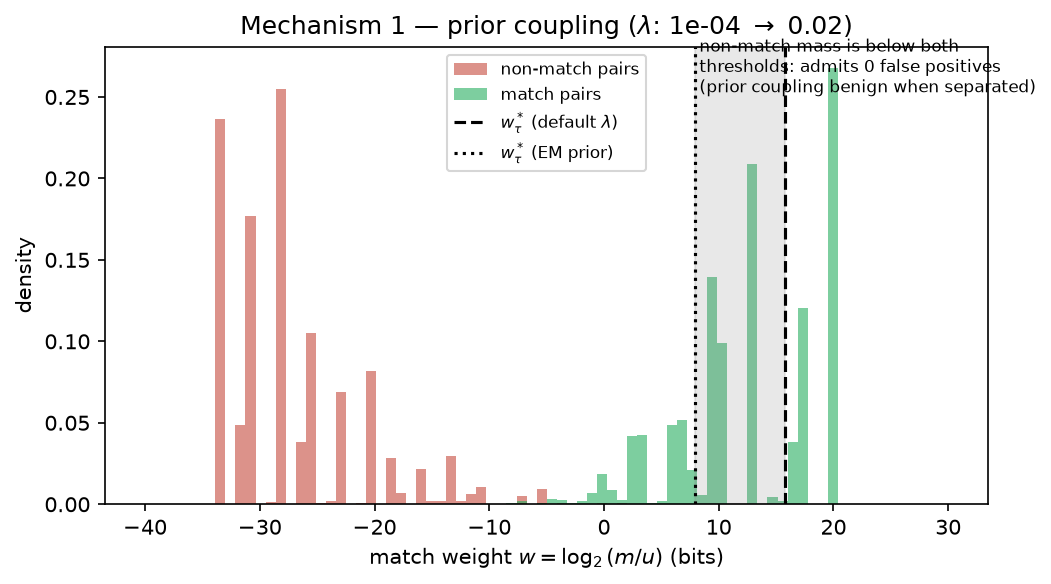
\includegraphics[width=0.86\textwidth]{figures/paradox_mech1.png}
\caption{Mechanism 1 (prior coupling) on NC-voter in posterior log-odds. The decision
threshold is fixed at $t=\log_2\frac{\tau}{1-\tau}=2.50$ bits; the EM-estimated prior
$\lambda\approx0.023$ shifts the non-match distribution up by $\Delta b\approx7.9$ bits
(grey to orange), admitting about 612 non-match pairs in the shaded band as false positives.
Prior coupling is secondary here to the Mechanism 2 recall collapse.}
\label{fig:mech1}
\end{figure}

\begin{figure}[h]
\centering
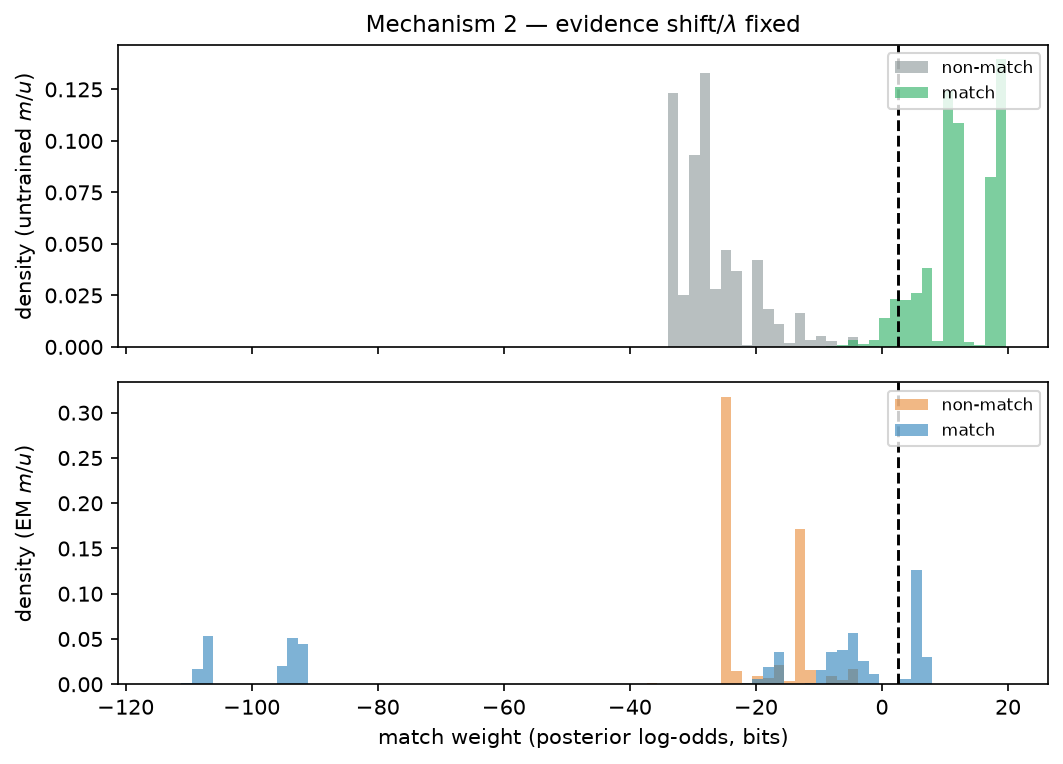
\includegraphics[width=0.86\textwidth]{figures/paradox_mech2.png}
\caption{Mechanism 2 (evidence shift) on NC-voter, $\lambda$ fixed at $10^{-4}$. Top panel:
untrained $m/u$ (match in green, non-match in grey); bottom panel: EM $m/u$ (match in blue,
non-match in orange). The EM-fitted weights move the match distribution sharply left
(median $12.7\to-8$ bits) while the non-match distribution moves only slightly right
($-28\to-24$), closing the separating gap; recall collapses as true matches are scored
toward non-match territory. Dashed line: fixed threshold $t$.}
\label{fig:mech2}
\end{figure}

For comparison, Figures~\ref{fig:mech1-synth} and~\ref{fig:mech2-synth} repeat the two
mechanisms on the synthetic duplicate-bearing benchmark of Section~\ref{sec:emp}, where the
paradox is measured. The EM-fitted prior is smaller there ($\lambda\approx0.0069$), so the
prior shift is $\Delta b\approx6.1$ bits and it admits only about $11$ non-match pairs in the
candidate set. The EM $m/u$ there \emph{increase} the match weights (median $17\to24$ bits)
and \emph{decrease} the non-match weights ($-25\to-38$), i.e.\ they \emph{widen} the
separating gap rather than collapse it. In this sample, therefore, neither mechanism
visibly floods the boundary: the EM degradation measured at scale is carried by prior
coupling admitting partial-collision non-matches at the higher duplicate density of the
100{,}000-record benchmark, which a 5{,}000-record sample under-represents. The core
takeaway stands: in both data sets the failure is a mismatch among the bundle
$(m/u,\lambda,\tau)$, and the same tandem calibration repair (Section~\ref{sec:alg}) applies.

\begin{figure}[h]
\centering
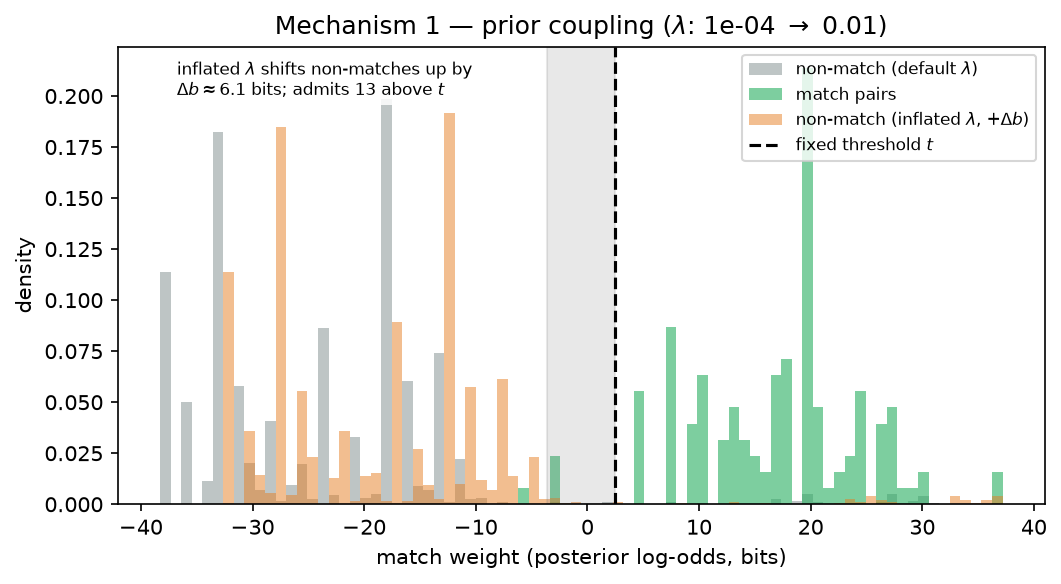
\includegraphics[width=0.86\textwidth]{figures/paradox_mech1_synth.png}
\caption{Mechanism 1 on the synthetic duplicate-bearing benchmark (posterior log-odds).
Threshold fixed at $t=2.50$ bits; EM's fitted prior $\lambda\approx0.0069$ shifts the
non-match distribution up by $\Delta b\approx6.1$ bits, admitting about 11 non-match pairs
in the shaded band.}
\label{fig:mech1-synth}
\end{figure}

\begin{figure}[h]
\centering
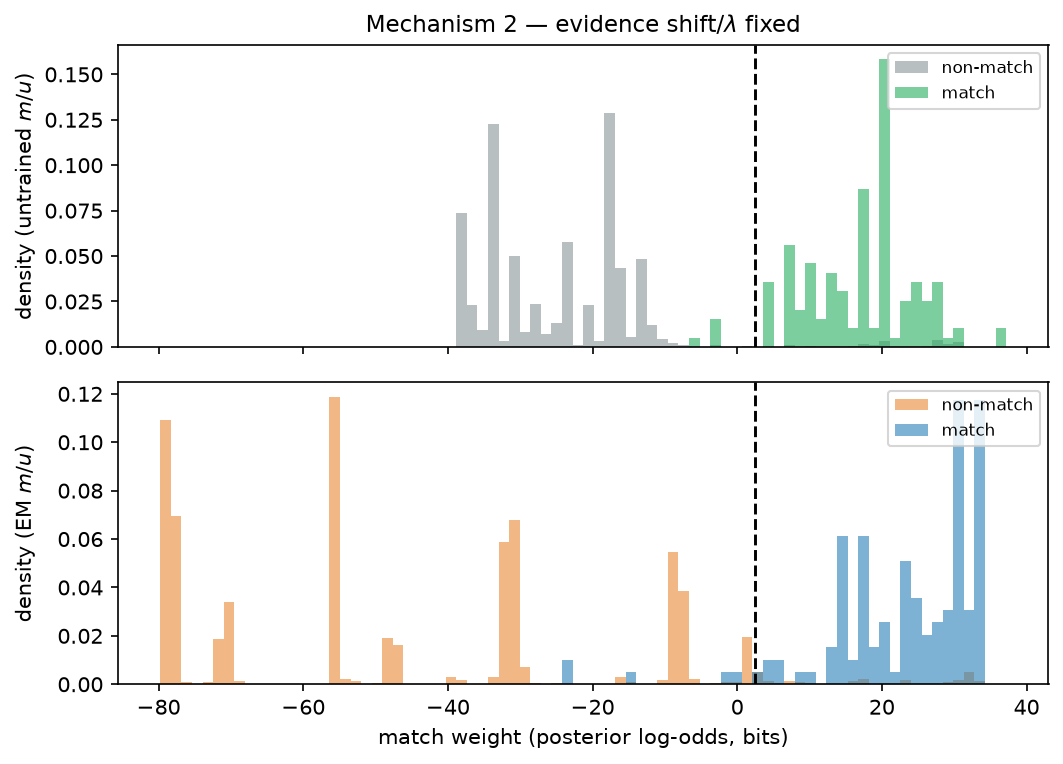
\includegraphics[width=0.86\textwidth]{figures/paradox_mech2_synth.png}
\caption{Mechanism 2 on the synthetic duplicate-bearing benchmark (top: untrained $m/u$;
bottom: EM $m/u$). The EM weights \emph{raise} match weights (median $17\to24$) and
\emph{lower} non-match weights ($-25\to-38$), widening the gap rather than collapsing it, so
Mechanism~2 is not the dominant failure on this data set.}
\label{fig:mech2-synth}
\end{figure}

\begin{table}[h]
\centering
\caption{Mutated NC-voter resolution at fixed $\tau=0.85$ (3{,}000 in-index, 1{,}500
positive, 1{,}500 negative queries). Date-of-birth and email comparisons are unavailable.}
\label{tab:real}
\begin{tabular}{lcccc}
\toprule
Configuration & Precision & Recall & Specificity & F1 \\
\midrule
Untrained defaults & 100.0\% & 85.6\% & 100.0\% & 92.2\% \\
Supervised $m/u$ & 99.9\% & 89.3\% & 99.9\% & 94.3\% \\
EM (free prior) & 73.7\% & 52.9\% & 81.1\% & 61.6\% \\
EM, prior reset to $10^{-4}$ & 100.0\% & 24.3\% & 100.0\% & 39.1\% \\
\bottomrule
\end{tabular}
\end{table}

Two findings qualify the synthetic result. First, on this harder real schema supervised
calibration does \emph{help}: it raises recall (85.6\% to 89.3\%) at virtually no cost to
precision (100.0\% to 99.9\%). The ``untrained defaults win'' claim in the synthetic
benchmark is therefore not universal; where partial agreement is genuinely informative,
trained $m/u$ can be better. Second, the \emph{unsupervised} (EM) result remains
catastrophic --- F1 collapses from 92.2\% to 61.6\% --- and, notably, resetting the EM prior
to $10^{-4}$ makes it \emph{worse} (39.1\%) by crushing recall. On this data EM's fitted
$m/u$ are themselves unreliable, so prior anchoring alone cannot repair them. The robust,
general conclusion is that freely fitting EM parameters is dangerous without joint
calibration, whereas supervised calibration transfers to a real schema and can be
beneficial; the two are not interchangeable remedies.

\subsection{Smoothing and regularisation}
\label{sec:smoothing}
A natural question is whether the genuine residual stems from noisy per-level probability
estimates, which regularisation could fix. If level $k$ of a comparison has $n_k$ observed
occurrences among a total of $N$ training pairs over $K$ levels, the empirical
$m$-probability is $\hat m_k=n_k/N$. Laplace (additive) smoothing, equivalently a Dirichlet
prior with concentration $\alpha$, replaces it by
\begin{equation}
\hat m_k^{(\alpha)}=\frac{n_k+\alpha}{N+K\alpha},
\end{equation}
which pulls the estimate toward the uniform value $1/K$ and removes zero counts. Because the
residual mechanism of Section~\ref{sec:paradox} is that trained models over-weight
partial-similarity levels, and those levels are precisely the ones where $n_k$ is large, one
might expect larger $\alpha$ to reduce the residual.

Table~\ref{tab:smooth} tests this on the supervised calibration of the 50{,}000-reference
benchmark at fixed $\tau$. Increasing $\alpha$ from 0.5 to 50 barely moves the supervised
F1 (94.4\% to 93.6\%), leaving a persistent gap of roughly four points below the untrained
defaults ($\approx98\%$). The residual is therefore not an artefact of level-count variance
or zero counts; it reflects a structural modelling choice --- the trained model rewards
partial-similarity agreement more than the default weight scheme does --- and smoothing the
level probabilities toward uniform does not reverse that choice. We therefore recommend
Laplace/Dirichlet smoothing as a variance remedy (and use it in our supervised estimator by
default), but stress that it does not, by itself, close the paradox; the repair remains the
joint $(\lambda,\tau)$ calibration of Section~\ref{sec:alg}.

It is natural to ask whether a \emph{non-symmetric} Dirichlet prior --- different
concentrations on the match and non-match probabilities, $\alpha_m\neq\alpha_u$ --- offers
additional protection against the evidence residual. Algebraically it can: the decision
depends only on the per-level ratio $m_k/u_k$ (via $w_k=\log_2(m_k/u_k)$), so shrinking
$m$ and $u$ toward different targets changes the effective weights. In particular, raising
the concentration on the \emph{mismatch} (else) level of $m$ more than that of $u$ dampens
the learned $m$ of the partial-similarity levels, which is precisely the mechanism behind the
residual of Section~\ref{sec:paradox}. However, two cautions apply from our experiments.
First, symmetric smoothing already spans $\alpha\in\{0.5,5,50\}$ with negligible effect on
F1, so any asymmetry would have to act strongly on the \emph{relative} shape of $m$ versus
$u$ to matter, not merely on the overall concentration. Second, because $w_k$ depends only
on the ratio, an asymmetric prior is operationally equivalent to a particular re-weighting of
the comparison levels, and must be re-validated together with $\lambda$ and $\tau$ (the
coherent-bundle rule). We therefore treat $\alpha_m\neq\alpha_u$ as an additional, principled
but data-dependent lever rather than a default remedy.

\begin{table}[h]
\centering
\caption{Supervised calibration of the synthetic benchmark at fixed $\tau=0.85$ under
Laplace smoothing $\alpha$. The untrained defaults give F1 $\approx98\%$ throughout.}
\label{tab:smooth}
\begin{tabular}{lccc}
\toprule
Smoothing $\alpha$ & 0.5 & 5 & 50 \\
\midrule
Supervised F1 & 94.4\% & 93.8\% & 93.6\% \\
\bottomrule
\end{tabular}
\end{table}

\subsection{Sensitivity of the threshold to prior misspecification}
\label{sec:sensitivity}
Equation \eqref{eq:threshold} makes the coupling explicit:
$w_\tau^*=t-b$, with $t=\log_2\frac{\tau}{1-\tau}$ and $b=\log_2\frac{\lambda}{1-\lambda}$.
If the true prior is $\lambda$ but the pipeline uses a misspecified $\tilde\lambda=c\lambda$,
the bias changes by
\begin{equation}
\Delta b=\log_2\frac{\tilde\lambda/(1-\tilde\lambda)}{\lambda/(1-\lambda)}
\;\approx\;\log_2 c\qquad(\lambda\ll 1).
\end{equation}
The simplification $\log_2 c$ is accurate in sparse entity-resolution settings, where both
$\lambda$ and $\tilde\lambda$ are small --- match rates below $10^{-2}$, as here
($\lambda=10^{-4}$) --- because $1-\lambda\approx1$ and $\log_2 c$ is then the dominant term;
it degrades only as $\lambda$ approaches a threshold-region prior of order $10^{-1}$.
To preserve the same effective threshold, $\tau$ must be adjusted by the same number of
bits: a factor $c$ in the prior requires an offset of $\approx\log_2 c$ in
$\mathrm{logit}_2(\tau)$. In fully unsupervised settings $\lambda$ cannot be estimated
reliably, so this relation bounds how much the operating point can move for a given prior
error.

Table~\ref{tab:sens} quantifies the consequence: the best F1 attainable after re-optimising
$\tau$ at each prior. The untrained model is stable (best F1 $0.98$--$1.00$) across two
orders of magnitude in $\lambda$; the EM model is highly sensitive, its attainable F1
falling from $0.96$ at $\lambda=10^{-5}$ to $0.81$ at $\lambda=10^{-2}$. Our guidance for the
unsupervised setting is therefore: (i)~prefer the default or blocking-adjusted prior rather
than a free EM estimate; (ii)~select $\tau$ on a validation split over a grid of candidate
$\lambda$; and (iii)~report the range of F1 across that grid as an explicit sensitivity
bound. A wide range (as for EM) is a warning that the configuration is unsafe without
labelled data.

\begin{table}[h]
\centering
\caption{Best F1 attainable after re-optimising $\tau$ at each assumed prior, on the
duplicate-bearing population. The optimal $\tau$ for every EM row is $0.98$.}
\label{tab:sens}
\begin{tabular}{lccc}
\toprule
Assumed $\lambda$ & $10^{-5}$ & $10^{-3}$ & $10^{-2}$ \\
\midrule
Untrained, best F1 & 0.99 & 0.99 & 0.98 \\
EM, best F1 & 0.96 & 0.91 & 0.81 \\
\bottomrule
\end{tabular}
\end{table}

\subsection{Additional metrics: calibration, discrimination, and cost}
\label{sec:metrics}
F1 at a single threshold does not separate ranking discrimination from probabilistic
calibration, nor does it reflect asymmetric false-positive/false-negative costs. We therefore
report three further quantities, evaluated pairwise over the blocked candidate pairs (which
is consistent with these metrics, and complements the query-level confusion matrices above):
the \emph{Brier score} (mean squared error of the match probability
$\frac1n\sum_i(p_i-y_i)^2$), the \emph{Average Precision} (area under the precision--recall
curve, a threshold-free measure of how well matches are ranked above non-matches), and the
\emph{expected decision cost} at the unit-cost-optimal threshold
$\tau^*=C_{FP}/(C_{FP}+C_{FN})$, together with pairwise F1 (Table~\ref{tab:metrics}).
Lower Brier and cost are better; higher Average Precision is better.

\begin{table}[h]
\centering
\caption{Pairwise evaluation metrics (untrained vs.\ EM) on both data sets. Brier and
expected cost: lower is better; Average Precision: higher is better.}
\label{tab:metrics}
\begin{tabular}{lcccc}
\toprule
 & \multicolumn{2}{c}{NC-voter} & \multicolumn{2}{c}{Synthetic} \\
\cmidrule(lr){2-3}\cmidrule(lr){4-5}
Metric & Untrained & EM & Untrained & EM \\
\midrule
Brier & 0.0009 & 0.0157 & 0.0254 & 0.0511 \\
Average Precision & 0.997 & 0.440 & 0.367 & 0.487 \\
F1 (pairwise) & 0.978 & 0.428 & 0.634 & 0.540 \\
Expected cost & 0.0009 & 0.0163 & 0.0250 & 0.0367 \\
$\tau^*$ (unit cost) & 0.81 & 0.07 & 0.93 & 1.00 \\
\bottomrule
\end{tabular}
\end{table}

On the NC-voter file the EM fit is worse on every quantity --- calibration (Brier
$0.0009\to0.0157$), discrimination (Average Precision $0.997\to0.440$), pairwise F1, and
expected cost --- consistent with the Mechanism~2 evidence collapse. On the synthetic
benchmark the picture is the precise mirror that exposes the paradox: EM \emph{improves}
ranking discrimination (Average Precision $0.367\to0.487$) while it \emph{worsens}
calibration (Brier $0.0254\to0.0511$) and, at the fixed $\tau$, pairwise F1
($0.634\to0.540$) and expected cost ($0.0250\to0.0367$, with the unit-cost-optimal threshold
moving from $0.93$ to $1.00$). Training can therefore sharpen how well the score ranks
matches above non-matches while still degrading the calibrated, operational outcome --- the
calibration paradox quantified with a metric that separates ranking from calibration.

\section{Related work}
The Fellegi--Sunter model \cite{fellegi1969} already framed linkage as a decision problem
with error-rate targets, and Winkler's line of work formalised optimal decision rules and
frequency-based parameter estimation \cite{winkler1993,winkler2000}. Christen's monograph
\cite{christen2012} surveys pragmatic threshold and calibration practice. The
precision--recall and threshold-selection literature \cite{davis2006} treats the operating
point as a tunable trade-off but, as far as we know, does not make explicit that $m/u$,
$\lambda$, and $\tau$ form a single coupled decision rule whose components cannot be
changed independently. The contribution here is that explicit log-odds decomposition
(\eqref{eq:logodds}--\eqref{eq:threshold}), the identification of prior coupling as the
dominant mechanism, and the tandem calibration procedure.

\section{Discussion and conclusion}
The calibration paradox is the statement that training the evidence parameters $m/u$ can
worsen a decision that already includes a prior $\lambda$ and a threshold $\tau$. The
log-odds decomposition shows why: the posterior log-odds is the sum of the evidence weight
$w$ and a prior bias $b=\log_2\frac{\lambda}{1-\lambda}$, and the decision compares this to
$t=\log_2\frac{\tau}{1-\tau}$. Retraining $m/u$ moves the evidence distribution; a freely
estimated prior moves the bias; a fixed $\tau$ holds the target fixed. Changing any one
without the other two relocates the operating point.

Two distinct mechanisms drive the observed drop. \emph{Prior coupling} is a global bias
shift: an EM prior inflated from $10^{-4}$ to $7.2\times10^{-3}$ lowers the effective weight
threshold by about $6$ bits and admits a flood of false positives; re-anchoring the prior
recovers most of the loss on the synthetic benchmark. \emph{The genuine residual} is a shift
of the non-match weight distribution caused by over-weighting partial-similarity levels,
which survives prior anchoring and keeps jointly re-optimised trained models slightly below
the defaults on the synthetic data. Real-data replication (Section~\ref{sec:real}) refines
this: supervised calibration can improve outcomes on harder schemas (it lifted NC-voter F1
from 92.2\% to 94.3\% at fixed $\tau$), whereas freely fitted EM remains catastrophically
miscalibrated. Smoothing the level probabilities (Section~\ref{sec:smoothing}) is a
valuable variance remedy but does not, by itself, close the residual; and the threshold is
explicitly sensitive to prior misspecification (Section~\ref{sec:sensitivity}), so a wide
F1 range across candidate priors is a warning sign in unsupervised settings.

The practical message is methodological: in a Fellegi--Sunter process, the triple
$(m/u,\lambda,\tau)$ is a \emph{coherent bundle}. Calibration is only meaningful when the
evidence, the prior bias, and the decision threshold are estimated and selected together,
and then evaluated on held-out data. Retraining $m/u$ while leaving $\lambda$ and $\tau$
unchanged is not a safe optimisation; it is a hidden change of operating point, and---for
unsupervised calibration especially---usually a worse one.

\begin{thebibliography}{9}
\bibitem{fellegi1969}
Ivan P. Fellegi and Alan B. Sunter.
\newblock A theory for record linkage.
\newblock Journal of the American Statistical Association, 64(328):1183--1210, 1969.

\bibitem{winkler1993}
William E. Winkler.
\newblock Improved decision rules in the Fellegi--Sunter model of record linkage.
\newblock In Proceedings of the Section on Survey Research Methods, American Statistical Association, pages 274--279, 1993.

\bibitem{winkler2000}
William E. Winkler.
\newblock Frequency-based matching in the Fellegi--Sunter model of record linkage.
\newblock Statistical Research Division, U.S. Bureau of the Census, Research Report Series RR2000/06, 2000.

\bibitem{christen2012}
Peter Christen.
\newblock Data Matching: Concepts and Techniques for Record Linkage, Entity Resolution, and Duplicate Detection.
\newblock Springer, 2012.

\bibitem{davis2006}
Jesse Davis and Mark Goadrich.
\newblock The relationship between precision-recall and ROC curves.
\newblock In Proceedings of the 23rd International Conference on Machine Learning, pages 233--240, 2006.

\bibitem{mclachlan2000}
Geoffrey McLachlan and David Peel.
\newblock Finite Mixture Models.
\newblock John Wiley \& Sons, 2000.

\bibitem{pipeline}
Denis Robert.
\newblock A two-stage entity resolution pipeline with FAISS blocking and Splink matching.
\newblock Technical report, Independent Researcher, 2026.
\end{thebibliography}

\appendix

\section{Estimation of $m$, $u$, and $\lambda$}
\label{app:estimation}
This appendix details how the three quantities of the decision rule
\eqref{eq:decision} are obtained, when labelled pairs are available and when they are not.

\subsection{Labeled estimation}
Suppose a set of labelled candidate pairs is split into true matches ($M$-pairs) and
non-matches ($U$-pairs). For a field with $K$ comparison levels, let $n_{k}^{M}$ and
$n_{k}^{U}$ count the pairs observed at level $k$, and let $N_M=\sum_k n_k^M$ and
$N_U=\sum_k n_k^U$. Under conditional independence the level probabilities are the
relative frequencies
\begin{equation}
\hat m_k=\frac{n_k^{M}}{N_M},\qquad \hat u_k=\frac{n_k^{U}}{N_U}.
\end{equation}
With Laplace (Dirichlet) smoothing of concentration $\alpha$ (Section~\ref{sec:smoothing}),
\begin{equation}
\hat m_k=\frac{n_k^{M}+\alpha}{N_M+K\alpha},\qquad
\hat u_k=\frac{n_k^{U}+\alpha}{N_U+K\alpha}.
\end{equation}
Non-symmetric versions use $\alpha_m$ and $\alpha_u$, respectively. The labelled sample also
yields a prior estimate $\hat\lambda=N_M/(N_M+N_U)$ from the match rate among candidate
pairs; this is the rate \emph{within the blocked candidate set} and, for a prior over
random pairs, must be corrected by dividing by the blocking recall
\cite{winkler2000}.

\subsection{Expectation-maximisation (unlabeled) estimation}
When no labels exist, the true match status of each candidate pair is a latent variable
$z_i\in\{M,U\}$. The EM algorithm iterates:
\begin{enumerate}
\item[\textbf{E-step.}] Using current estimates $(\hat m,\hat u,\hat\lambda)$, compute the
posterior probability that pair $i$ is a match from \eqref{eq:posterior}, equivalently from
the log-odds decomposition \eqref{eq:logodds}.
\item[\textbf{M-step.}] Re-estimate the level probabilities as \emph{expected} relative
frequencies,
\begin{equation}
\hat m_k=\frac{\sum_{i}\mathbb E[ \mathbf 1_{\{z_i=M\}}]\mathbf 1_{\{k_i=k\}}}{N_M'},
\end{equation}
with $N_M'=\sum_i \mathbb E[\mathbf 1_{\{z_i=M\}}]$ a weighted total, and similarly for
$u_k$; and update the prior as
\begin{equation}
\hat\lambda=\frac{1}{n}\sum_i\mathbb E[\mathbf 1_{\{z_i=M\}}],
\end{equation}
the expected match proportion among the $n$ candidate pairs. The cycle is repeated to a
fixed point.
\end{enumerate}

Note that in this pipeline EM is run on the comparison vectors of the \emph{blocked
candidate pairs} --- the top-$k$ nearest neighbours of each record --- not on all possible
pairs. The algorithm treats these pairs as given, so the fitted $u$ and $\lambda$ are
\emph{candidate-space} quantities: the non-match component is dominated by near-collisions
that resemble true matches, which is precisely why the fitted classes overlap and reproduce a
narrow gap. This is a property of the input candidate set, not of the EM update itself; when
a random-pair prior is required, the blocking-adjusted prior of Section~\ref{sec:alg}
converts $\lambda$ accordingly.

Three remarks connect this to the paradox. First, the free estimate in the M-step reflects
the \emph{blocked candidate} mix, not the random-pair base rate: candidate sets are drawn
from records that already resemble each other, so $\hat\lambda$ drifts upward --- this is the
source of the prior coupling of Section~\ref{sec:paradox}. Dividing by blocking recall, or
holding $\lambda$ fixed at a prior estimate, corrects it. Second, only the ratios $m_k/u_k$
enter the decision, and EM additionally fixes the overall scale relative to $\lambda$; both
the scale and $\lambda$ jointly set the operating point, so neither can be changed
independently of $\tau$. Third, richer estimators --- frequency-based refinement of $m/u$
\cite{winkler2000}, or regularised and Bayesian variants of EM \cite{mclachlan2000} ---
modify the M-step but leave the coupling of Section~\ref{sec:paradox} intact. The tandem
calibration of Section~\ref{sec:alg} is the layer that reconciles whatever estimator is used
with a chosen $\tau$.

\section*{Use of Artificial Intelligence}
During the preparation of this work the author used an AI coding and writing assistant (the
DeepSeek V4 Flash 0731 large language model) to assist with drafting and editing the
manuscript and preparing the experiments. The tool was not listed as an author. The
theoretical derivation and all reported results were reviewed and verified by the author,
who takes full responsibility for the content, including any remaining errors and/or omissions.

\end{document}